%++++++++++++++++++++++++++++++++++++++++
% Don't modify this section unless you know what you're doing!
\documentclass[letterpaper,12pt]{article}
\usepackage{tabularx} % extra features for tabular environment
\usepackage{amsmath}  % improve math presentation
\usepackage{graphicx} % takes care of graphic including machinery
\usepackage[margin=1in,letterpaper]{geometry} % decreases margins
\usepackage{cite} % takes care of citations
\usepackage[final]{hyperref} % adds hyper links inside the generated pdf file
\usepackage{pgfplotstable, booktabs}
\usepackage{placeins}
\usepackage{tabularray}
\usepackage{titlesec}
\usepackage{fancyhdr}
\usepackage{empheq}
\usepackage{amssymb}
\usepackage{sectsty}
\usepackage{tcolorbox}
\usepackage{listings}
\usepackage{xcolor}
\usepackage{parskip}
\usepackage{siunitx}
\usepackage{cancel}
\usepackage{enumitem}

\definecolor{codegreen}{rgb}{0,0.6,0}
\definecolor{codegray}{rgb}{0.5,0.5,0.5}
\definecolor{codepurple}{rgb}{0.58,0,0.82}

\lstdefinestyle{mystyle}{
    commentstyle=\color{codegreen},
    keywordstyle=\color{codepurple},
    numberstyle=\tiny\color{codegray},
    stringstyle=\color{codegreen},
    basicstyle=\ttfamily\small,
    breakatwhitespace=false,         
    breaklines=true,                 
    captionpos=b,                    
    keepspaces=true,                                                     
    showspaces=false,                
    showstringspaces=false,
    showtabs=false,                  
    tabsize=4
}

\lstset{style=mystyle}
  
\newcommand*\widefbox[1]{\fbox{\hspace{0em}#1\hspace{0em}}}

\pagestyle{fancy}
\fancyhf{} % Clear all header and footer fields
\fancyhead[L]{MEC E 331}
%\fancyhead[C]{Center Header}
\fancyhead[C]{Assignment 2}
\fancyhead[R]{Alex Diep}

\fancyfoot[C]{\thepage}

\pgfplotsset{compat=1.18} 
\titleformat*{\section}{\Large\bfseries}
\titleformat*{\subsection}{\large\bfseries}

\renewcommand{\thesection}{Question \arabic{section}}
\renewcommand{\thesubsection}{(\alph{subsection})}

\hypersetup{
	colorlinks=true,       % false: boxed links; true: colored links
	linkcolor=blue,        % color of internal links
	citecolor=blue,        % color of links to bibliography
	filecolor=magenta,     % color of file links
	urlcolor=blue         
}
%++++++++++++++++++++++++++++++++++++++++
\begin{document}
% \begin{titlepage}
%     \centering
%     \vspace*{2cm} % Adjust vertical spacing
    
%     % Title
%     \Huge {MEC E 301 \\Lab 1: Dimensional Measurement} \\
%     \vspace{1cm} % Adjust vertical spacing
    
%     % Author
%     \Large by: Alex Diep \\
%     \vspace{1cm} % Adjust vertical spacing

%     % Date
%     \Large Date: September 19, 2023 \\ % or manually specify a date
%     \vspace{4cm} % Adjust vertical spacing

%     % CCID and Student ID in smtaller font
%     \normalsize CCID: abdiep \\
%     \normalsize Student ID: 1664334 \\ 
%     \normalsize Section: D21 \\
    
%     \vfill % Fill vertical space
    
%     % Additional content (e.g., university logo or other information)
    
% \end{titlepage}
\renewcommand\arraystretch{1.5}

\section{}
A tube acts as a water siphon. Determine the speed of jet and the
minimum pressure of water in the bend (at the point A).

\begin{figure}[h]
    \centering
    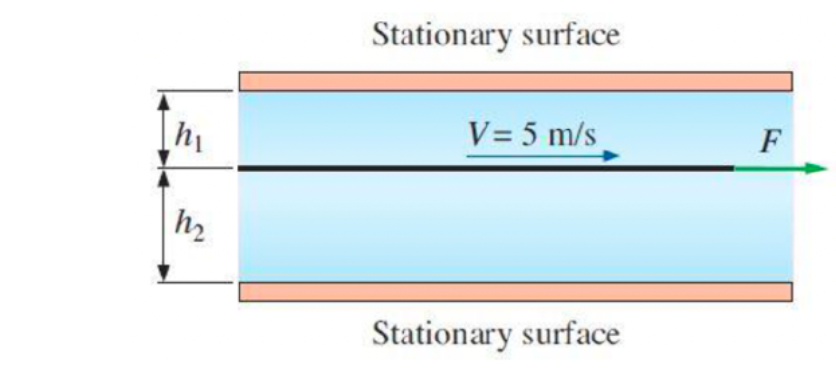
\includegraphics[width=0.5\linewidth]{Questions/Figures/Q1ProblemDiagram.png}
    \caption{Tube with water siphon}
    \label{fig:Q1ProblemDiagram}
\end{figure}

\textbf{Solution} \\
Assumptions:
\begin{itemize}
    \item Steady flow
    \item Incompressible flow
    \item Negligible viscous effects
    \item Negligible diameter change
    \item Reservoir is large enough to be considered infinite
\end{itemize}

By the Bernoulli equation, the speed of jet is given by:
\begin{gather*}
    \underbrace{\cancel{\frac{P_1}{\rho} - \frac{P_2}{\rho}}}_{\text{Both exposed to atm}} + \frac{v_2^2}{2} - \underbrace{\cancel{\frac{v_1^2}{2}}}_{\text{large reservoir}} + g(z_2 - z_1) = 0 \\
    \frac{v_2^2}{2} + g(z_2 - z_1) = 0 
\end{gather*}

Which results in
\begin{align*}
    v_2 &= \sqrt{2g(z_1 - z_2)} \\
    &= \sqrt{2(9.81)(7)} \\
    &= \boxed{\qty{11.7}{\meter\per\second}}
\end{align*}

In the pipe, by the assumptions, the velocity is constant. Therefore taking the Bernoulli equation between the pipe exit and the bend, 
\begin{gather*}
    \frac{P_A}{\rho} - \frac{P_2}{\rho} + \cancel{\frac{v_A^2}{2} - \frac{v_2^2}{2}} + g(z_A - z_2) = 0 \\
    \frac{P_A}{\rho} - \frac{P_2}{\rho} + g(z_A - z_2) = 0 \\
\end{gather*}

Rearranging for $P_A$,
\begin{align*}
    P_A &= \rho g(z_2 - z_A) + P_2 \\
    &= (1000)(9.81)(-7 - 1) + 101325 \\
    &= \boxed{\qty{22.84}{\kilo\pascal}}
\end{align*}
\section{}
% Question 2 of 3 (15 marks): The � velocity component of a steady, two-dimensional 
% incompressible flow field is � = 3��! − 2���, where � and � are constants. Velocity component 
% � is unknown. Generate an expression for � as a function of � and �.

The $x$ velocity component of a steady, two-dimensional incompressible flow field is $u = 3ax^2 - 2bxy$, where $a$ and $b$ are constants.
The $y$ velocity component $v$ is unknown. Generate an expression for $V$ as a function of $x$ and $y$.

\textbf{Solution:} \\
For an incompressible flow, $\nabla \cdot \vec{V} = 0$. Therefore,
\begin{align*}
    \frac{\partial u}{\partial x} + \frac{\partial v}{\partial y} &= 0 \\
    \frac{\partial}{\partial x} (3ax^2 - 2bxy) + \frac{\partial v}{\partial y} &= 0 \\
    6ax - 2by + \frac{\partial v}{\partial y} &= 0 \\
    \frac{\partial v}{\partial y} &= 2by - 6ax \\
    v &= by^2 - 6axy + f(x)
\end{align*}
Therefore, 
\begin{empheq}[box=\fbox]{align*}
    \vec{V} &= (3ax^2 - 2bxy) \hat{i} + (by^2 - 6axy + f(x)) \hat{j}
\end{empheq}
\section{}
The system shown in the figure is used to accurately measure changes when the pressure 
is increased by $\Delta P$ in the water pipe. When $\Delta h = 70$ mm, what is the change 
in the pipe pressure?

\begin{figure}[h]
    \centering
    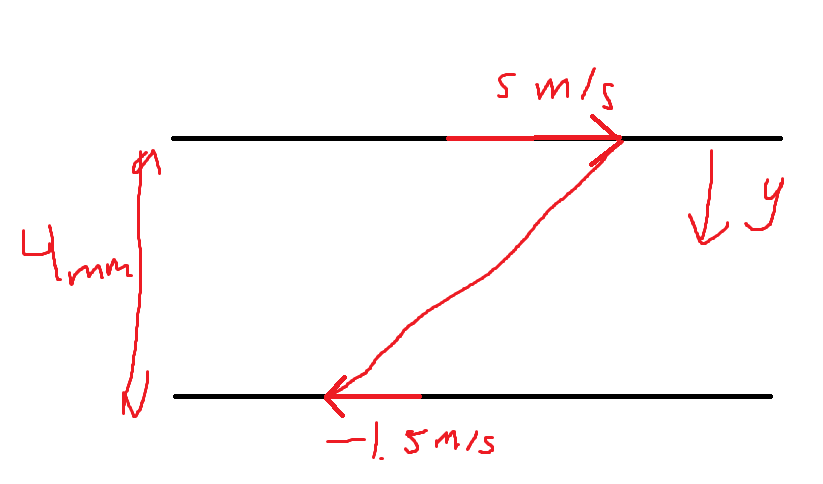
\includegraphics[width=0.3\textwidth]{Questions/Figures/Q3ProblemDiagram.png}
    \caption{Convoluted manometer diagram}
    \label{fig:Q3ProblemDiagram}
\end{figure}

Assumptions:
\begin{itemize}
    \item $x$ is less than $l$
    \item Density is constant
    \item The manometer is open to the atmosphere
\end{itemize}

By conservation of mass, the volume displaced on the right side of the manometer is equal to the volume displaced on the left side of the manometer. 

\begin{align}
    \Delta V_{left} &= \Delta V_{right} \nonumber \\
    \Delta h \left(\frac{\pi}{4} D_{right}^2\right) &= x \left(\frac{\pi}{4} D_{left}^2\right) \nonumber \\
    \implies x &= \Delta h \left(\frac{D_{right}}{D_{left}}\right)^2 \label{eq:Q3x} \nonumber \\
    &= 70 \times \left(\frac{3}{30}\right)^2 \nonumber \\
    &= \qty{0.7}{\milli\meter} \nonumber
\end{align}

In the initial state, the pressure balance going from the water to the air is (look at where the fluid starts and ends; 
downwards displacement is positive, upwards displacement is negative):
\begin{equation}
    P_{w, 1} + \rho_{w} g h_1 + \rho_{g} g (h_2 - h_1) = P_{atm} \label{eq:Q3State1}
\end{equation}

In the final state, the pressure balance is:
\begin{equation}
    P_{w, 2} + \rho_{w} g (h_1 + x) + \rho_{g} g (h_2 - \Delta h - x - h_1) = P_{atm} \label{eq:Q3State2}
\end{equation}

Subtracting (\ref{eq:Q3State1}) from (\ref{eq:Q3State2}) yields:
\begin{equation}
    P_{w, 2} - P_{w, 1} = -\rho_{w} g x + \rho_{g} g (\Delta h + x) \label{eq:Q3DeltaP}
\end{equation}

To find the density of glycerin given SG = 1.26, we can use the following equation:
\begin{equation}
    \rho_{g} = \rho_{H_2O} \times SG = 1000 \times 1.26 = \qty{1260}{\kilogram\per\meter\cubed} \nonumber
\end{equation}

Substituting this into (\ref{eq:Q3DeltaP}) yields:
\begin{equation}
    \Delta P = -1000 \times 9.81 \times \frac{0.7}{1000} + 1260 \times 9.81 \times \frac{70 + 0.7}{1000} = \boxed{\qty{867.0}{\pascal}} \nonumber
\end{equation}
\section{}
Consider a cylinder rolling on a board, with a torque applied to the latter:
\begin{figure}[h]
    \centering
    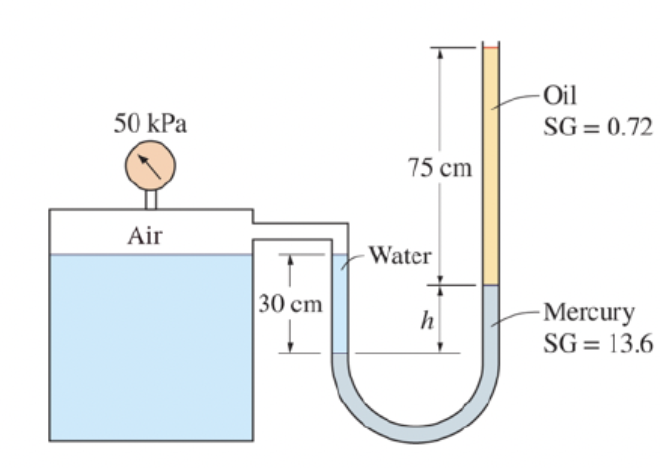
\includegraphics[width=0.5\textwidth]{Questions/Figures/Q4ProblemDiagram.png}
    \caption{Cylinder rolling on a board.}
    \label{fig:Q4 System}
\end{figure}

% As shown, the angle of tilt is denoted by θ, the torque applied to the board is τ , and q measures the
% distance the cylinder rolls down the board. Let J denote the mass moment of inertia of the board
% about its pivot and Jc, Rc and Mc the mass moment of inertia, radius and mass of the cylinder,
% respectively. Assuming roll without slip, the equations of motion can be shown to be
% write in mathmode

As shown, the angle of tilt is denoted by $\theta$, the torque applied to the board is $\tau$, and $q$ 
measures the distance the cylinder rolls down the board. Let $J$ denote the mass moment of inertia of the board 
about its pivot and $J_c$, $R_c$ and $M_c$ the mass moment of inertia, radius and mass of the cylinder, 
respectively. Assuming roll without slip, the equations of motion can be shown to be:

\begin{align}
    &\left(\frac{J_c}{R_{c}^2} + M_c\right)\ddot{q} + M_{c}g \sin{\theta} - M_{c}q \dot{\theta}^2 = 0 \label{eq: Q4a1} \\
    &(M_{c}q^2 + J + J_c)\ddot{\theta} + 2M_{c}q \dot{q} \dot{\theta} + M_{c}gq \cos{\theta} = \tau \label{eq: Q4a2}
\end{align}

\subsection{}
\textit{What is the order of this system?}

The system consists of two 2nd order differential equations, so the order of the system is 2.
\subsection{}
\textit{Defining $x = (q, \theta, \dot{q}, \dot{\theta})$, $u = \tau$ and $y = q$, write the state model of this system.}

Isolating the $\ddot{q}$ and $\ddot{\theta}$ terms in (\ref{eq: Q4a1}) and (\ref{eq: Q4a2}) respectively, we get:

\begin{align*}
    \ddot{q} &= \frac{1}{\frac{J_c}{R_{c}^2} + M_c} \left(M_{c}q \dot{\theta}^2 - M_{c}g \sin{\theta}\right) \\
    \ddot{\theta} &= \frac{1}{M_{c}q^2 + J + J_c} \left(u - 2M_{c}q \dot{q} \dot{\theta} - M_{c}gq \cos{\theta}\right)
\end{align*}

The state model is therefore:
\begin{empheq}[box=\fbox]{align*}
    \dot{x} &=
    \begin{bmatrix}
        \dot{q} \\
        \dot{\theta} \\
        \frac{1}{\frac{J_c}{R_{c}^2} + M_c} \left(M_{c}q \dot{\theta}^2 - M_{c}g \sin{\theta}\right) \\
        \frac{1}{M_{c}q^2 + J + J_c} \left(u - 2M_{c}q \dot{q} \dot{\theta} - M_{c}gq \cos{\theta}\right)
    \end{bmatrix} \\
    y &= q
\end{empheq}

\subsection{}
\textit{Does the system in (b) have a state-space form? Why or why not?}

The system in (b) does not have a state-space form because the state dynamics are not linear due to the presence of 
the $q^2$, $\sin{\theta}$, $\cos{\theta}$, $\theta^2$, $2M_{c}q \dot{q} \dot{\theta}$, and various other non-linear terms.
    
        


% \section{}
A steady, incompressible, two-dimensional velocity field is given by $\vec{V} = (0.523 - 1.88x + 3.94y)\hat{i} 
+ (-2.44 + 1.26x + 1.88y)\hat{j}$, calculate the acceleration at the point $(x, y) = (-1.55, 2.07)$.

Since $\vec{V} = \langle u, v \rangle$ is a function of $(x, y, t)$, the acceleration is given by the multivariable chain rule:
\begin{align}
    \vec{a} &= \frac{\partial \vec{V}}{\partial t} \cancel{\frac{d t}{d t}} + 
    \frac{\partial \vec{V}}{\partial x} \frac{d x}{d t} +
    \frac{\partial \vec{V}}{\partial y} \frac{d y}{d t} \nonumber \\
    & = \cancel{\frac{\partial \vec{V}}{\partial t}} +
    \frac{\partial \vec{V}}{\partial x} u + 
    \frac{\partial \vec{V}}{\partial y} v \nonumber \\
    & = 
    \begin{bmatrix}
        -1.88 \\
        1.26
    \end{bmatrix}
    u +
    \begin{bmatrix}
        3.94 \\
        1.88
    \end{bmatrix}
    v \nonumber \\
\end{align}

Plugging in the given values to evaluate for $u$ and $v$ at the point $(x, y) = (-1.55, 2.07)$:
\begin{align}
    u &= 0.523 - 1.88(-1.55) + 3.94(2.07) \nonumber \\
    &= 11.5928 \nonumber \\
    v &= -2.44 + 1.26(-1.55) + 1.88(2.07) \nonumber \\
    &= -0.5014 \nonumber
\end{align}

Evaluating for acceleration:
\begin{empheq}[box=\fbox]{align}
    \vec{a} &= 
    \begin{bmatrix}
        -23.77 \\
        13.66 
    \end{bmatrix}
    [\hat{i} + \hat{j}] \nonumber 
\end{empheq}

% \newpage
% %\bibliographystyle{IEEEtran}
% %\bibliography{citations.bib}
% %\bibliography{}

% \newpage
% \appendix
% \sectionfont{\large}
\section{Appendix: Matplotlib Python Code to Render Graphs}
This is just some random code.
\begin{lstlisting}[language=Python]
if transactions: Transaction.create_transactions() # if transactions = "true"
node.generate_emptyState() # empty state for all nodes
S.initial_events() # initiate initial events to start with

while not queue.isEmpty() and clock <= targetTime:
    next_e = queue.get_next_event()
    clock = next_e.time # move clock to the time of the event
    Event.execute_event(next_e)
    Queue.remove_event(next_e)

print results
\end{lstlisting}

\end{document}